\chapter{Frapi v1: sharing FENCE data}
\label{chap3}

\section{Introduction}

In March 2019, the Glance Team started to develop \textbf{\acrshort{frapi}} (\textbf{F}ENCE \textbf{R}EST \textbf{API}), a library to help developers address the need to expose data to CAP and other CERN services via REST APIs. Due to the nature of the problem, the first version aimed to make information available and did not focus on receiving and writing information.

The idea was to create a solution that was part of FENCE, the framework used by all the team's systems at the time. Followed by FENCE principles, Frapi's initial release was based primarily on using JSON configuration files and FacTree integration. The following sections describe how the first version of Frapi was developed, the integration with FENCE, and the usage by Glance applications and external services.

\section{Slim micro-framework}

A fundamental task of a REST API server is routing, in other words, deciding which parts of the program should be executed given a request to a specific endpoint. It was the skeleton of the Frapi module with the other features developed around it. Knowing the importance of routing and after learning from past mistakes of creating in-house solutions and reinventing the wheel, it was decided to use an already developed solution and extend it according to the custom needs of Glance systems.

The constraints formulated by the team were that it should be a library with complete documentation and good community support. Those requirements aimed to rely on a highly used software, increasing the quality of the final product and reducing the learning curve due to extensive documentation and plugins, examples and answers from the community. Additionally, the package should support PHP 5.4, the current version of the programming language used by FENCE on production at the time.

With the constraints in mind, Slim \cite{slim-website} was the chosen library among Lumen \cite{lumen-website}, Mezzio\cite{mezzio-website}, Laravel\cite{laravel-website} and Symfony \cite{symfony-website}. It is a PHP micro framework that helps developers quickly write simple APIs. Micro framework means that it does not include many features of full-fledged frameworks, focusing on receiving HTTP requests, routing and returning an HTTP response. Of the considered packages, Slim \cite{slim-website} had more usage by other projects and no dependency on full-stack frameworks, such as Laravel \cite{laravel-website} and Symfony \cite{symfony-website}. Usage and community support were measured with the number of downloads on the Composer package manager \cite{composer-website}, GitHub stars and questions with an answer on StackOverflow.

Even though Slim was already on version 3, Frapi used the previous library version since the new one did not support PHP 5.4. Considering that was on the team's plans to update to PHP 7 on the FENCE systems, an abstraction was created on top of Slim 2 \cite{slim-2-doc} to emulate the interfaces from Slim 3 and ease a future migration.

\section{Installation}
\label{sec:frapi-v1-installation}

For developers wishing to use the first version of Frapi to provide a REST API, the requirements were to use FENCE, which was the case for all Glance systems and create an \texttt{/api} folder with a PHP file as the entry point, JSON file with settings and an Apache configuration for redirection \cite{frapi-v1-setup-documentation}.

\begin{figure}
\centering
\begin{minipage}{0.9\textwidth}
    \dirtree{%
    .1 service-work/.
    .2 api/.
    .3 index.php.
    .3 api.json.
    .3
    \vdots.
    .2 htaccess.
    .2
    \vdots.
    }
\end{minipage}
\caption{Example of the directory structure of a system built with Frapi v1.}
\label{fig:frapi-v1-directory-structure}
\end{figure}

The file tree of the system should look like \autoref{fig:frapi-v1-directory-structure}, consisting of the \texttt{api} directory with the \texttt{index.php} file (\autoref{code:frapi-v1-index-php}) working as the REST API entry point. In essentially 3 lines, it imports dependencies, initialises Frapi with the path of the configuration file and starts the API service.

\begin{listing}[H]
\begin{minted}{php}
<?php

require_once "./vendor/autoload.php";

$api = new \Fence\Frapi\Api("api.json");

$api->run();
\end{minted}
\caption{Script executed when any REST API request arrives at the server.}
\label{code:frapi-v1-index-php}
\end{listing}


The \texttt{api.json} file (\autoref{code:frapi-v1-api-json}) supports multiple API settings that will be later explained in detail on \autoref{sec:creating-endpoints}. The only mandatory value is the user class, which defines the authentication method used and can be later customised. For new applications using CERN's Keycloak \cite{keycloak-website} authentication, the base class \texttt{KeycloakUser} is enough.

\begin{listing}[htbp]
\begin{minted}{json}
{
    "user": {
        "class": "Fence\\Frapi\\Users\\KeycloakUser"
    }
}
\end{minted}
\caption{Minimal configuration for Frapi v1.}
\label{code:frapi-v1-api-json}
\end{listing}

The last requirement is the \texttt{.htaccess} (\autoref{code:frapi-v1-htaccess}) Apache configuration. It is common between systems using Frapi and contains request redirection used by Slim and enables the \texttt{Authorization} header used on authentication which will be further explained on \autoref{sec:frapi-v1-auth}.

\begin{listing}[htbp]
\begin{minted}{apache}
# Required for Slim Framework
RewriteEngine on
RewriteCond %{REQUEST_FILENAME} !-d
RewriteCond %{REQUEST_FILENAME} !-f
RewriteRule . index.php [L]

# Enable authorization header
RewriteCond %{HTTP:Authorization} ^(.*)
RewriteRule .* - [e=HTTP_AUTHORIZATION:%1]
\end{minted}
\caption{Apache configuration for redirecting request to the API entry point.}
\label{code:frapi-v1-htaccess}
\end{listing}

\section{Creating endpoints}\label{sec:creating-endpoints}

Frapi v1 supports creating FacTree-based and custom endpoints by defining them on JSON format. After defining a new route, the configuration should be added to JSON file and referenced on the API settings as exemplified on code \autoref{code:api-json-files}. If desired, all endpoint definition files on specific folders can be parsed by Frapi as shown on \autoref{code:api-json-folders}.

\begin{listing}[htbp]
\begin{minted}{json}
{
	"endpoints": {
	    "files": [ "routes/task.json" ]
	}
}
\end{minted}
\caption{Frapi v1 configuration for parsing endpoint files.}
\label{code:api-json-files}
\end{listing}

\begin{listing}[htbp]
\begin{minted}{json}
{
	"endpoints": {
		"folders": [ "routes" ]
	}
}
\end{minted}
\caption{Frapi v1 configuration for parsing all endpoint files inside a directory.}
\label{code:api-json-folders}
\end{listing}

\subsection{FacTree endpoints}

At first, Frapi supported the FENCE micro-ORM by providing automatic routes to all FacTree models. However, it became an issue due to the lack of control over what was being exposed to an external system. The solution was to define, as endpoint settings, the resources to be exposed. Glance developers could expose information to be consumed by external systems by configuring routes without writing a single PHP line of code.

Using Service Work as an example, a collaboration \texttt{Task} represents work to be done during the year. Each task has one \texttt{Activity}, which is a way to categorise them as illustrated in \autoref{fig:class-diagram-sw-task}. With a FacTree model already in place, a FENCE developer can expose task data on a new route by adding an endpoint setting as exemplified by \autoref{code:task-factree-endpoint-settings}.

\begin{figure}[htbp]
  \centering
  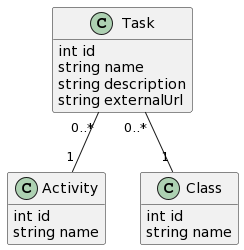
\includegraphics[scale=0.77]{Imagens/chap03/class-diagram-sw-task.png}
  \caption{Simplified class diagram from the Service Work \texttt{Task}, \texttt{Activity} and \texttt{Class} models.}
  \label{fig:class-diagram-sw-task}
\end{figure}

\begin{listing}[htbp]
\begin{minted}{json}
{
    "type": "factree",
    "path": "/tasks",
    "factory": {
        "name": "sw-task",
        "path": "/src",
        "order": {
            "__components__": [
                "name",
                "description"
            ],
            "activity": {
                "__components__": [
                    "name"
                ]
            }
        }
    },
    "response": {
        "objectName": {
            "single": "task",
            "multiple": "tasks"
        }
    }
}
\end{minted}
\caption{FacTree endpoint configuration file for the \texttt{Task} model.}
\label{code:task-factree-endpoint-settings}
\end{listing}

The parameter \texttt{type} indicates Frapi to interpret the settings as a FacTree endpoint. The URI path of the route is defined on \texttt{path}. In this case, a client can request a list of all tasks by sending a \texttt{GET} request to https://alice-glance.cern.ch/service-work/api/tasks.

The data returned by the endpoint and FacTree are configured under the \texttt{factory} key.  The combination of \texttt{name} and \texttt{path} defines the factory file and its path, meaning that Frapi will try to find the FacTree definitions on \texttt{api/src/factories/sw-task.json} (\autoref{fig:frapi-v1-factree-dir}). The \texttt{order} parameter configures which fields are returned on the HTTP response. In the example, the \texttt{/tasks} endpoint returns only the task's name, description and the name of the activity. External URL and class information are hidden from the API consumer. Task and activity IDs are also returned by default.

\begin{figure}
\centering
\begin{minipage}{0.9\textwidth}
    \dirtree{%
    .1 api/.
    .2 routes/.
    .3 tasks.json.
    .3
    \vdots.
    .2 src/.
    .3 factories/.
    .4 sw-task.json.
    .4
    \vdots.
    .2 api.json.
    .2
    \vdots.
    }
\end{minipage}
\caption{Directory structure for defining FacTree endpoints with Frapi v1.}
\label{fig:frapi-v1-factree-dir}
\end{figure}

Finally, the last configuration parameter defines the format of the response. When requesting a single task (\autoref{code:request-single-task}), the response contains a \texttt{task} with a data object as the value. On the other hand, while requesting all tasks (\autoref{code:request-all-tasks}), the output changes to \texttt{tasks} key with a list of objects as values.

\begin{listing}[htbp]
\begin{minted}{text}
GET /api/tasks/197

200 OK
{
	"task": {
		"id": 197,
		"name": "Resource Coordinator",
		"description": "Responsible for...",
		"activity": { "id": 2, "name": "Management" }
	}
}
\end{minted}
\caption{Example of HTTP request and response from a FacTree endpoint to a single task.}
\label{code:request-single-task}
\end{listing}

\begin{listing}[htbp]
\begin{minted}{text}
GET /api/tasks

200 OK
{
	"tasks": [
		{
			"id": 197,
			"name": "Resource Coordinator",
			"description": "Responsible for...",
			"activity": { "id": 2, "name": "Management" }
		},
		{ ... },
		{ ... },
		...
	]
}
\end{minted}
\caption{Example of HTTP request and response from a FacTree endpoint to all tasks.}
\label{code:request-all-tasks}
\end{listing}

\subsection{Custom endpoints}
\label{sec:custom-endpoints}

By providing only FacTree endpoints, Frapi supported exclusively read operations. Clients could consume Glance data, but creating, updating and deleting resources was not yet supported. Since the in-house ORM did not fully support \acrfull{crud} operations, Frapi needed another route creation method for the unsupported scenarios. The solution was to create custom endpoints where the developer could programmatically handle the request data and return the response. Due to the solution's flexibility, all CRUD operations could be supported.

The definition of a custom endpoint on Frapi is done similarly to a FacTree endpoint: by creating a JSON configuration file. In this case, the code \autoref{code:custom-endpoint-json} exemplifies the two parameters needed: a class type and the class's namespace.

\begin{listing}[htbp]
\begin{minted}{json}
{
    "type": "class",
    "class": "Alice\\ServiceWork\\Api\\CreateTask"
}
\end{minted}
\caption{Configuration file for custom endpoints.}
\label{code:custom-endpoint-json}
\end{listing}

After defining the route, the developer should create the corresponding class as illustrated in code \autoref{code:custom-endpoint-php}. The class should extend Frapi's \texttt{BaseEndpoint} abstract class and implement the method \texttt{buildEndpoints()}  where the developer can add any custom code to read the request and write a response. Frapi exposes the instance of the Slim router via \texttt{getSlim()} from \texttt{BaseEndpoint}, and it is used in this example to define a \texttt{POST /tasks} endpoint for creating tasks. All Slim v2 features \cite{slim-2-doc} are available through the same interface. The endpoint's behaviour is defined on the second argument \texttt{post()} as an anonymous function. In the example, a Slim v3 forward-compatible request object is provided by Frapi and used to create a task. Finally, the \texttt{render} utility function returns a 201 HTTP response to the client with the associative array serialised as JSON on the body and a \texttt{Content-Type: application/json} header.

\begin{listing}[htbp]
\begin{minted}{php}
<?php

namespace Alice\ServiceWork\Api;

use Fence\Frapi\Endpoints\BaseEndpoint;

class CreateTask extends BaseEndpoint
{
    public function buildEndpoints()
    {
        $this->getSlim()->post(
            "/tasks",
            function () {
			    $request = $this->getApi()->getRequest();

                $newTask = $this->createTask($request);

                $this->getApi()->render(["task" => $newTask], 201);
            }
        );
    }

    private function createTask($request)
    {
        // Crates task based on request data...
    }
}
\end{minted}
\caption{PHP class with the custom endpoint definition for creating a Service Work task.}
\label{code:custom-endpoint-php}
\end{listing}

\section{Environment variables}

Glance systems usually need previously defined values that affect how the program works, for example, database credentials, paths on the filesystem used by the application, secrets and running mode (development or production). FENCE stores those values on \texttt{configuration.json} files, which are parsed when the framework is initialised and made available as global variables.

To address the issue of using global variables described in \autoref{sec:global-variables}, Frapi started to rely on environment variables \cite{frapi-environment-variables}, which were independent of the framework in use and could be set in multiple ways, including the operating system scope. To use an environment variable anywhere on the codebase, a single line of code (\autoref{code:getenv-php}) is needed.

\begin{listing}[htbp]
\begin{minted}[startinline]{php}
$databasePassword = getenv("DB_PASSWORD");
\end{minted}
\caption{Example of retrieving an environment variable on PHP.}
\label{code:getenv-php}
\end{listing}

There are multiple ways to define an environment variable \cite{defining-environment-variables}. However, Frapi also manages to automatically parse a set of files on the root of the API folder and make the values available through the application. The solution was inspired by how the Vue framework \cite{vue-about} handles environment variables \cite{vue-environment-variables}.

The files automatically parsed by Frapi are listed below, where \texttt{[mode]} can be \texttt{development}, \texttt{integration} and production \texttt{production}.

\begin{itemize}
    \item \texttt{.env}: loaded in all cases
    \item \texttt{.env.local}: loaded in all cases, ignored by VCS (version control system)
    \item \texttt{.env.[mode]}: only loaded in the specified mode
    \item \texttt{.env.[mode].local}: only loaded in the specified mode, ignored by VCS
\end{itemize}

\texttt{.env}, also called \textit{dotenv}, files are commonly used on the industry application and contain a key-value list of user-defined variables, as illustrated on code \autoref{code:dotenv-example}. Notice that the \texttt{LOG\textunderscore DIR} and \texttt{OUTPUT\textunderscore DIR} keys reference \texttt{BASE\textunderscore PATH}, avoiding duplication of values.

\begin{listing}[htbp]
\begin{minted}{bash}
# .env
DB_USERNAME="alice-service-work"
DB_PASSWORD="my-super-secret"

BASE_PATH="/svr/alice/service-work"
LOG_DIR="${BASE_PATH}/logs"
OUTPUT_DIR="{BASE_PATH}/output"
\end{minted}
\caption{Example of a \texttt{.env} file.}
\label{code:dotenv-example}
\end{listing}

An environment file for a specific mode (e.g. \texttt{.env.production}) will take higher priority than a generic one (e.g. \texttt{.env}). Local files (e.g. \texttt{.env.local}) will take higher priority than the committed ones (e.g. \texttt{.env}). The following list enumerates the loading order of \textit{.env} files. Every time an environment file is loaded, existing variables are overwritten by the new ones.

\begin{enumerate}
    \item \texttt{.env}
    \item \texttt{.env.local}
    \item \texttt{.env.[mode]}
    \item \texttt{.env.[mode].local}
\end{enumerate}

Some environment variables, such as secrets, should not be committed to the version control system. For this case, an \texttt{.env.local} file should be used instead and ignored by \acrshort{vcs}.

\section{Authentication and Authorisation}
\label{sec:frapi-v1-auth}

It is usual among software programs to limit actions according to the user roles. The same occurs on Glance applications. On Service Work, for example, only the Service Work Coordinator or the Resource Coordinator should be able to create and plan tasks, and only Project Leaders can assign members to a task. In this scenario, authentication and authorisation play a central role. The former verifies who the user is and determines whether they are who they claim to be. The latter verifies data the user can or cannot access and actions that are permitted \cite{auth0-authentication-authorization}. Usually, authentication occurs before authorisation.

During the development of Frapi, CERN was changing its \acrfull{sso} solution, transitioning from Shibboleth \cite{shibboleth-website} to Keycloak \cite{keycloak-website}. SSO affects how users are authenticated, and due to the duality of methods, Frapi supports both. To choose the authentication method, the application should define on the API configuration file a user class from Frapi's defaults \texttt{ShibbolethUser} and \texttt{KeycloakUser} or an extension of one of them.

\begin{listing}[htbp]
\begin{minted}{json}
{
    "user": {
        "class": "\\Fence\\Frapi\\Users\\KeycloakUser"
    },
    "endpoints": {
        "files": [],
        "folders": ["routes"],
    }
}
\end{minted}
\caption{Example of API configuration file using Keycloak authentication.}
% \label{}
\end{listing}

Both \texttt{KeycloakUser} and \texttt{ShibbolethUser} contain base user data such as CERN Person ID, name, email and username. CERN e-groups are also supported but fetched differently in each authentication scenario.

\subsection{Shibboleth authentication}

Configured and used by default on Glance servers, the SSO solution dating from 2008 used the Shibboleth Service Provider module for Apache and Microsoft \acrshort{adfs} (\acrlong{adfs}) to authenticate users using a single platform \cite{shibboleth-article}. After authentication, variables were set with the information of the current user. When defined on the API configuration, the \texttt{ShibbolethUser} class reads the variables when it is instantiated. The e-groups in which the user participates are also set as environment variables and parsed by the user class.

With the first version of CERN SSO, the mechanism for authenticating HTTP API users was using cookies generated at CERN servers. This was an issue since the Glance APIs were meant to be used by clients worldwide via their browsers or other CERN apps, independently of being hosted or not at CERN servers. The Glance team made an early attempt to solve this issue by performing its authentication. This was not an ideal solution due to the lack of experience of the developers in this area with such security risks.

\subsection{Keycloak authentication}

Due to a 20-fold increase in Microsoft license costs, the \acrshort{malt} (\acrlong{malt}) \cite{malt} \cite{malt-internal} \cite{malt-auth} project kicked off with one of its tasks to migrate CERN's Identity and Access Management solution, including single sign-on, to open source software. The chosen alternative was the Keycloak SSO, with a pilot release in 2019 \cite{keycloak-article}. It fitted Glance's needs, and the team was one of the early adopters of the service, developing the new API and back-end structures alongside the evolution of the Authorisation Service.

Different from Shibboleth, Glance systems should follow additional steps to use Keycloak. First, an application should be registered on the applications portal and enable \acrshort{oidc} (\acrlong{oidc}) \cite{registering-application} \cite{cern-auth-oidc-guide}. The registration will result in a \textit{client ID} and a \textit{client secret} that should be included on an \texttt{.env.local} file under the \texttt{CLIENT\textunderscore ID} and \texttt{CLIENT\textunderscore SECRET} keys.

API consumers acting on behalf of the user authenticates through the CERN Authorization Service, which verifies the user credentials. The client can use any of the OAuth grant types \cite{oauth-grant-type} in this step.  In case of success, the Authorization Service responds with an access token as a \acrfull{jwt}. JWT is an open standard defined by RFC 7519 \cite{rfc-7519} for securely transmitting JSON objects between parties in a compact and self-contained way that can be used on HTTP environments \cite{jwt-introduction}. The tokens are composed of a header, payload and signature, each base64 encoded and separated by dots. The payload contains a JSON object with useful data about the user that can later be used for authorisation. The signature is the output of the encryption of the header and payload parts.

% TODO: fig exemplo jwt em b64

After receiving the access token, the client should send it on every request to the API in the \texttt{Authorization} header using the \texttt{Bearer} schema. In this way, the server can verify who the user is and control access to resources.

% TODO: fig diagrama auth

When configured for Keycloak, Frapi reads the access token from the request header and uses the signature to verify if the message was not modified and check against CERN Authorization Service, the true issuer of JWT. These two steps guarantee the security of the API since no attacker can create fake tokens or change existing ones. After successful validation, the class \texttt{KeycloakUser} is instantiated with the data of the JWT payload and made available to be used by the API developers, including information about user roles. If an invalid token is provided, the API responds with \texttt{401} HTTP status code and an error message.

The new SSO solution, however, did not support e-groups, a fundamental information used by Glance for authorisation. To bypass this situation, the class \texttt{KeycloakUser} gets e-group information on demand via CERN WebServices. To use this feature, Glance systems should define the \texttt{WEBSERVICES\textunderscore LOGIN} and \texttt{WEBSERVICES\textunderscore PWD} environment variables with the credentials of the e-groups web service.

\subsection{Authorisation}
\label{sec:frapi-v1-authorisation}

With users authenticated, Frapi verifies whether they can access the resources of the endpoint. The authorisation was developed to be independent of the authentication method or SSO, working similarly for Shibboleth and Keycloak. Frapi parses the access criteria defined by the API developer and validates the current user object against it. If authorisation fails, Frapi responds to the client with \texttt{403 Forbidden} status code and an error message.

For FacTree endpoints, the permission schema should be added to the route JSON configuration, as illustrated in code \autoref{code:factree-auth}. In the example, it is defined under the \texttt{authorization} key as a list of rules for accessing the endpoint with the list of Service Work tasks. Frapi parses each rule as a single criteria and applies an OR boolean operator between them. In this case, the user needs to have either an \textit{admin} role \textbf{or} being a \textit{service-work-coordinator} within the \textit{cern-member} \textbf{and} \textit{alice-member} e-groups. Behind the scenes, the getter methods of the user object are used to validate the permissions. In the example, \texttt{\$user->getRoles()} and \texttt{\$user->getEgroups()} are used. Besides e-groups and roles, any custom user property is supported on the permission schema, needing only the user object to provide a corresponding getter method returning a list of strings.

\begin{listing}[htbp]
\begin{minted}{json}
{
    "type": "factree",
    "path": "/tasks",
    "authorization": [
        { "roles": ["admin"] },
        {
	        "egroups": ["cern-member", "alice-member"],
	        "roles": ["service-work-coordinator"]
	    }
    ],
    "factory": { "...": "..." }
}
\end{minted}
\caption{Access control configuration for a FacTree endpoint.}
\label{code:factree-auth}
\end{listing}

A similar logic applies to custom routes. The difference is that authorisation rules are listed on the corresponding PHP class. The code \autoref{code:php-auth} illustrates how to define the same set of rules of the previous example when registering a task by using the \texttt{authorize()} method from the \texttt{BaseEndpoint} abstract class.

\begin{listing}[htbp]
\begin{minted}[startinline]{php}
public function buildEndpoints()
{
    $this->getSlim()->post(
        "/tasks",
        $this->authorize([
            [ "roles" => ["admin"] ],
            [
                "egroups" => ["cern-member", "alice-member"],
                "roles"   => ["service-work-coordinator"],
            ],
        ]),
        function () {
            // Register task...
        }
    );
}
\end{minted}
\caption{Access control configuration for a custom endpoint.}
\label{code:php-auth}
\end{listing}

\subsection{User endpoint}

With the decoupling of the front and back end, the user interfaces developed by Glance became separate applications and consumers of the team APIs. One of the first needs of the clients was to retrieve experiment or system-specific information about the current user that was not available via the authentication methods.

\begin{listing}[htbp]
\begin{minted}{json}
{
	"personId": 837034,
	"username": "mgunters",
	"email": "mario.simao@cern.ch",
	"fullName": "Mario Gunter Simao",
	"firstName": "Mario",
	"lastName": "Gunter Simao",
	"egroups": ["alice-member", "fence-developers"],
	"role": ["developer"]
}
\end{minted}
\caption{Response example of the \texttt{/user} endpoint.}
\label{code:user-endpoint-response}
\end{listing}


Frapi exposes by default a \texttt{GET /user} endpoint, which returns information about the current user as shown on code \autoref{code:user-endpoint-response}. For custom properties, Frapi systems should extend the user class, implement getter methods and list the additional properties to be returned by the API under the \texttt{endpoints/user/additionalProperties} key as illustrated on \autoref{code:custom-props-json} and \autoref{code:custom-props-php}. The example shows how to add an \texttt{internalId} property to the current user endpoint.

\begin{listing}[htbp]
\begin{minted}{json}
{
    "user": {
        "class": "\\Alice\\ServiceWork\\User"
    },
    "endpoints": {
        "folders": [ "routes" ],
        "user": {
            "additionalProperties": [
                {
                    "key": "internalId",
                    "getter": "getInternalId"
                }
            ]
        }
    }
}
\end{minted}
\caption{Configuration for additional properties on the user endpoint.}
\label{code:custom-props-json}
\end{listing}

\begin{listing}[htbp]
\begin{minted}[startinline]{php}
class User extends \Fence\Frapi\Users\KeycloakUser
{
	private $internalId;

	public function __construct($token)
	{
		parent::__construct($token);

		// Fetch Internal ID...
	}

    public function getMemberId()
    {
        return $this->intenralId;
    }
}
\end{minted}
\caption{Custom \texttt{User} class with additional properties.}
\label{code:custom-props-php}
\end{listing}

\subsection{Logging}

In multi-user software, keeping a log of events such as errors, warnings, or other information is important to monitor the system's operation, debug problems and audit \cite{logging-wikipedia}. For the same reasons, having a logging mechanism that worked for Frapi was essential. The chosen solution was FENCE Logger due to the fact of being independent of the framework, worked well on previous applications and was already known by the Glance Team. The \texttt{Fence\textbackslash Logger} is a simple class with static methods (\autoref{code:logger-php-example}) for different log levels (debug, info, notice, warning, error, critical, alert and emergency) which writes messages as new lines on logfiles (\autoref{code:log-line-example}).

\begin{listing}[htbp]
\begin{minted}[startinline]{php}
\Fence\Logger::info("User logged in.");
\end{minted}
\caption{How to write logs on Frapi v1.}
\label{code:logger-php-example}
\end{listing}

\begin{listing}[htbp]
\begin{minted}{php}
[21-May-2023 22:43:42 Europe/Zurich] [INFO] User logged in.
\end{minted}
\caption{Example of a log line.}
\label{code:log-line-example}
\end{listing}

Like FENCE, when Frapi receives a request, it writes the first logs on the \texttt{api.log} file. After authentication, all the subsequent messages are written on a file named with the CERN username of the current user. The path where logfiles are saved is defined via the \texttt{LOG\textunderscore PATH} environment variable. To avoid large logfiles, Glance machines are configured with Logrotate \cite{logrotate-man} to chunks and compress old logs and facilitate the reading of recent ones.

\subsection{Error handling}
\label{sec:error-handling}

When a program encounters a runtime error, it is expected to be treated and properly inform the user about the issue. Whenever an unhandled exception was thrown on FENCE applications, the framework would display a generic HTML page informing the user about an unexpected error. It would email the developers with details and a complete stack trace. This solution did not fit Frapi's needs, mainly because it needed to return errors as JSON, the format used by the API consumers. Secondly, the strategy to send a new email on every unhandled error was problematic. It was common for developers to get their inboxes spammed by the same exceptions, and it was hard to monitor how much and how often errors occurred.

To address the issues above, Frapi implemented a new error handler \cite{frapi-error-handler-doc}. Unhandled exceptions are caught, logged, and the API responds with the \texttt{500 Internal Server Error} status code and the body of code \autoref{code:error-500-body}. The \texttt{id} field is a unique identifier of the error instance, which can be found on the user log file. The error response follows the JSON:API specification, which defines how REST APIs clients and servers should communicate \cite{json-api-intro} \cite{json-api-error} \cite{json-api-error-example}.

\begin{listing}[htbp]
\begin{minted}{json}
{
    "id": "5e417eec56914",
    "errors": [
        {
            "status": 500,
            "title": "Internal Error",
            "detail": "An unexpected server error occurred."
        }
    ]
}
\end{minted}
\caption{HTTP response when Frapi catches an unhandled exception.}
\label{code:error-500-body}
\end{listing}

To collect, manage and alert the developers about untreated exceptions, Frapi optionally supports Sentry \cite{sentry-about}. Sentry is a third-party error monitoring \acrshort{saas} (\acrlong{saas}) made available by the CERN IT team \cite{sentry-cern}. To send exceptions to the tool, the API should be configured with the URL of a Sentry instance, as exemplified in code \autoref{code:sentry-config}.

\begin{listing}[htbp]
\begin{minted}{json}
{
    "sentry": {
        "dns": "https://public@sentry.example.com/1"
    },
    "user": { },
    "endpoints": { }
}
\end{minted}
\caption{API configuration to enable Sentry.}
\label{code:sentry-config}
\end{listing}

Software errors, however, are not exclusively made of unexpected exceptions. There are cases where the application validates user input, checks domain invariants and others. In these scenarios, it is important to inform the API client about the error cause. As a solution, Frapi supports custom errors thrown as an instance of the \texttt{Fence\textbackslash Frapi\textbackslash Exceptions\textbackslash BaseException} class.

\autoref{code:custom-error-example} exemplifies how to throw custom errors to be formatted by Frapi in a scenario where Service Work tasks can not be created on weekends and should not have an empty name. In case of any validation error, the \texttt{BaseException} is thrown, automatically caught by Frapi and returned to the client, following the JSON:API specification as illustrated on \autoref{code:custom-error-response-example}. Custom errors are not automatically logged and are not sent to Sentry.

\begin{listing}[htbp]
\begin{minted}[startinline]{php}
$this->getSlim()->post("/tasks", function () {
	$request = $this->getApi()->getRequest();
	$errors = [];

	if ($this->isNameEmpty($request)) {
        $source = (new BaseSource())
            ->setPointer("/data/attributes/name");

		$emptyNameError = new BaseError();
		$emptyNameError
			->setStatus(StatusCodes::BAD_REQUEST)
			->setCode(1234) // Internal error code
			->setSource($source)
			->setTitle("Invalid Attribute")
			->setDetail("Name can not be empty.");

		$errors[] = $emptyNameError;
	}

	if ($this->isWeekend()) {
		$weekendError = new BaseError();
		$weekendError
			->setStatus(StatusCodes::FORBIDEN)
		    ->setDetail("Not allowed on Weekends.");

		$errors[] = $weekendError
	}

	if (count($errors) > 0) {
        $status = StatusCodes::BAD_REQUEST
		$exception = new BaseException($status);
		$exception->setErrors($errors);

		throw $exception;
	}

	// Register task...
});
\end{minted}
\caption{How to throw custom errors to be formated in user-friendly responses.}
\label{code:custom-error-example}
\end{listing}

\begin{listing}[htbp]
\begin{minted}{json}
{
    "errors": [
        {
            "status": "403",
            "detail": "Editing is not authorized on weekend."
        },
        {
            "status": 400,
            "code": 1234,
            "source": { "pointer": "/data/attributes/name" },
            "title": "Invalid Attribute",
            "detail": "Name can not be empty."
        }
    ]
}
\end{minted}
\caption{HTTP response body of custom errors following the JSON:API schema.}
\label{code:custom-error-response-example}
\end{listing}

\section{The Middleware pattern}
\label{sec:middleware}

The Middleware pattern, also known as the Chain of Responsibility \cite{chain-of-responsibility}, is a design pattern in which receiver objects, called middleware, are linked as a chain. Each receiver processes the message and calls the next one. Middleware can also interrupt the chain if needed, for example, when an error occurs. Slim supports the pattern \cite{slim-middleware-doc} and it is widely used by Frapi to orchestrate some of its core features via the Setup, Authentication and Endpoints Builder middleware.

\autoref{fig:frapi-internal-sequence} is a simplified sequence diagram of how Frapi works internally. When a client sends an HTTP request to the API server, Frapi is instantiated, loads files and setups essential services such as logger and error handler. Then, the middleware chain is called, starting with the Setup and following to Authentication and Endpoints Builder. After the sequence of receivers has finished their job, Slim maps the requested route to the correct function, which reads the request and sets the response object on Frapi, which outputs it to the server. Finally, the server returns an HTTP response to the API consumer.

\begin{figure}[htbp]
  \centering
  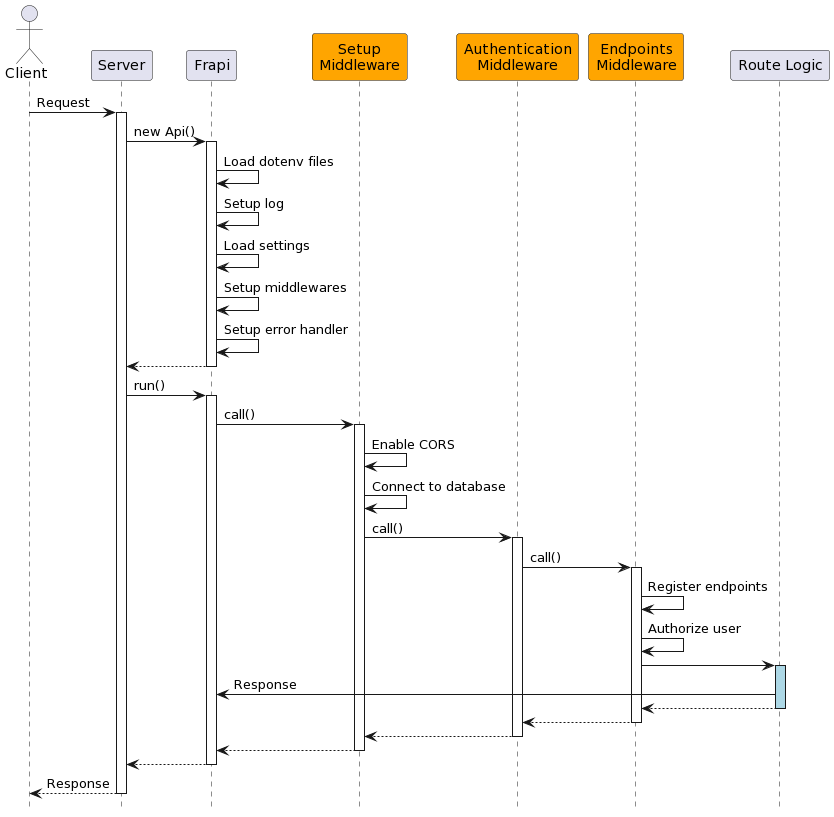
\includegraphics[scale=0.5]{Imagens/chap03/middleware-sequence-diagram.png}
  \caption{Sequence diagram of Frapi's internal call stack, including middleware.}
  \label{fig:frapi-internal-sequence}
\end{figure}